% The document class marks this as a poster, supplying various options that
% control rendering of some standard features (e.g., the title bar).

\documentclass[ % the name of the author
                    author={Dominic Moylett},
                % the name of the supervisor (preferably including title)
                supervisor={Dr. Raphael Clifford, Dr. Markus Jalsenius and Dr. Ben Sach},
                % the thesis    title (which cannot be blank)
                     title={An Empirical Analysis of Data Streaming Algorithms},
                % the thesis subtitle (which can    be blank)
                  subtitle={},
                % the degree programme (from BSc, MEng, MSci, MSc and PhD)
                    degree={MEng},
                % the year of submission
                      year={2014} ]{poster}

\usepackage{graphicx}

\begin{document}

% -----------------------------------------------------------------------------

\begin{frame}{} 

\vfill

\begin{columns}[t]
  \begin{column}{0.900\linewidth}
  \begin{block}{\Large Introduction}
  In the wake of Big Data, a large amount of recent research in Theoretical Computer Science has been focused on the data streaming model. Under this model, the computer only has access to a window of the input at any time, and the objective is to compute the solution with a sublinear amount of space. There have been a number of theoretical developments in Data Streaming in recent years, but very few of these have ever been implemented to see if they are practical.\\
  \vspace{\baselineskip}
  I have implemented two algorithms in C for stream-based pattern matching. Note the standard notation for pattern matching, where $m$ is the length of the pattern and $\Sigma$ is the alphabet:
  \begin{enumerate}
  \item An algorithm for parameterised matching with $O(m + \pi)$ space and $O(\log\pi)$ amortised time per character, where $\pi=min(m, \left|\Sigma\right|)$ by Amir et al.\footnote{Alphabet Dependence in Parameterized Matching by Amihood Amir, Martin Farach and S. Muthukrishnan}
  \item An algorithm for exact matching with $O(\log m)$ space and $O(1)$ time per character by Breslauer and Galil,\footnote{Real-Time Streaming String-Matching by Dany Breslauer and Zvi Galil} and deamortised by Simon's Algorithm.\footnote{String Matching Algorithms and Automata by Imre Simon} Sublinear space is achieved via Karp-Rabin fingerprints.
  \end{enumerate}

  \noindent
  All of these algorithms have been tested on 50MB of English text from the Pizza and Chili Corpus.
  \end{block}
  \end{column}
\end{columns}

\vfill

\begin{columns}[t]
  \begin{column}{0.422\linewidth}
  \begin{block}{\Large Parameterised Matching Results}
  \begin{center}
  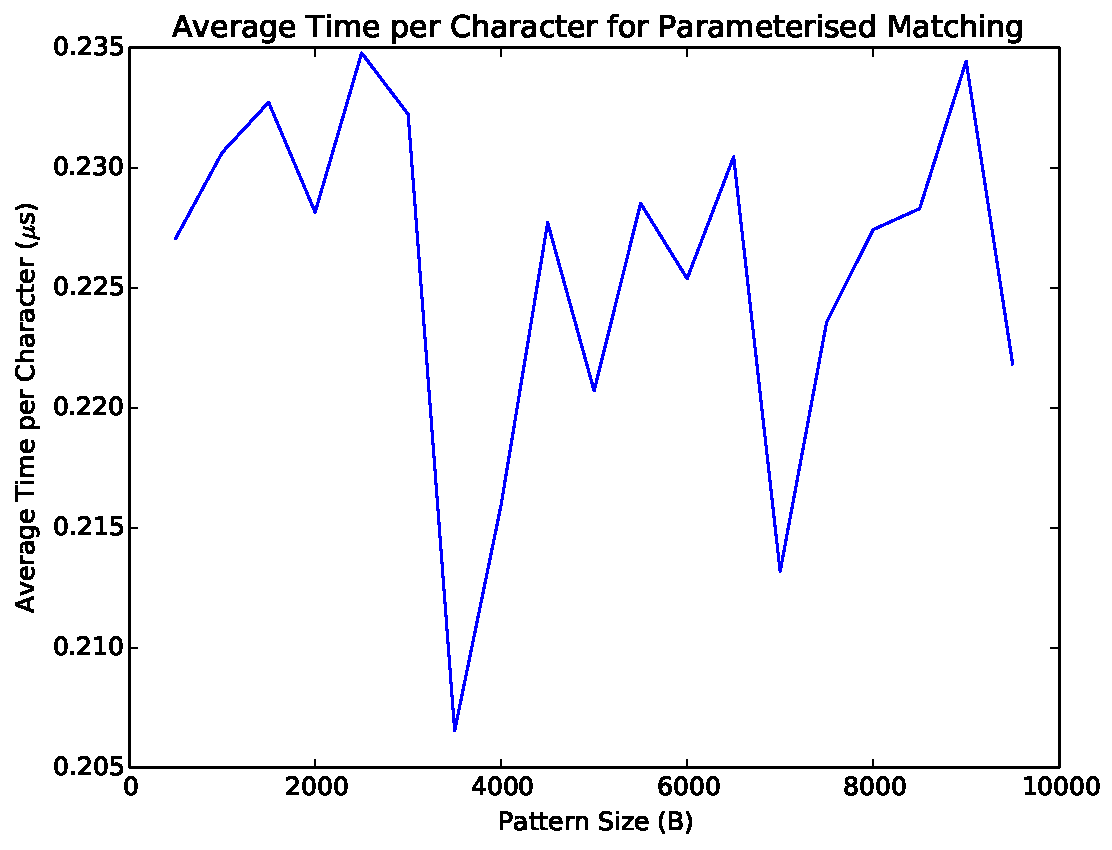
\includegraphics[scale=0.58]{parameterised_run_time}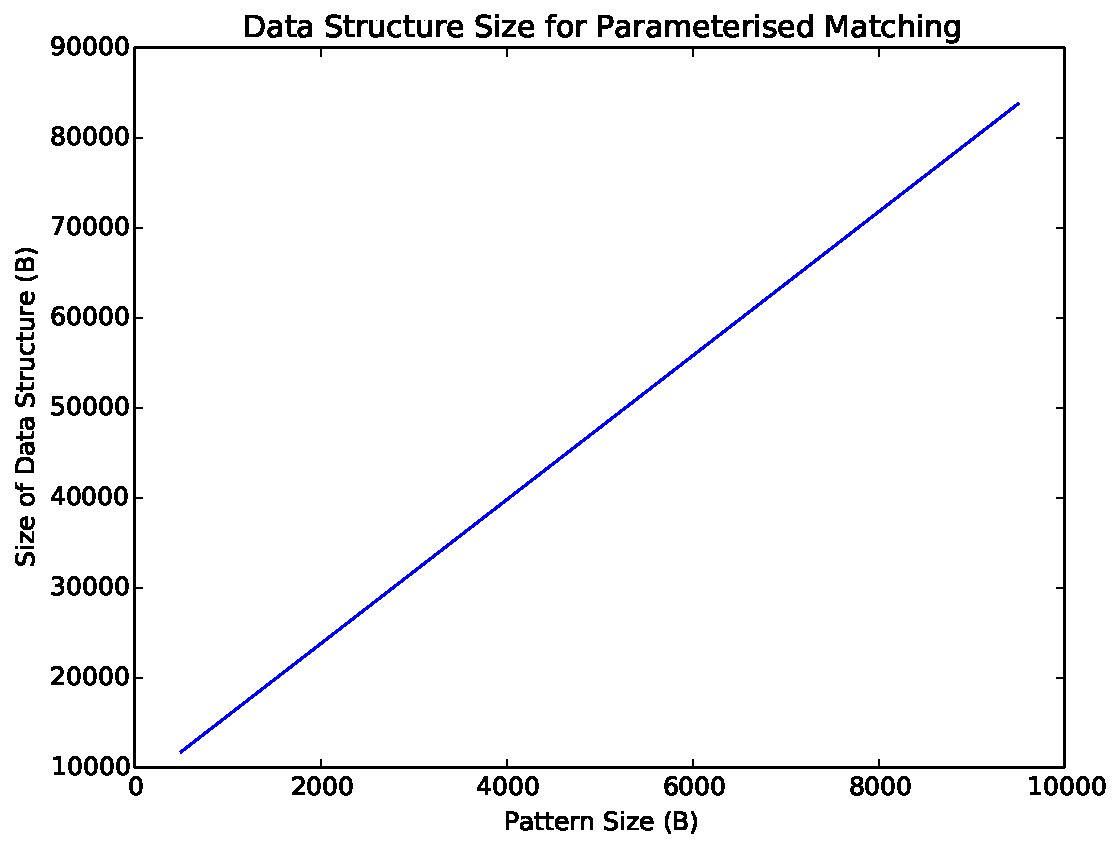
\includegraphics[scale=0.58]{parameterised_size}
  \end{center}
  \end{block}
  \end{column}

  \begin{column}{0.422\linewidth}
  \begin{block}{\Large Results for Exact Matching}
  \begin{center}
  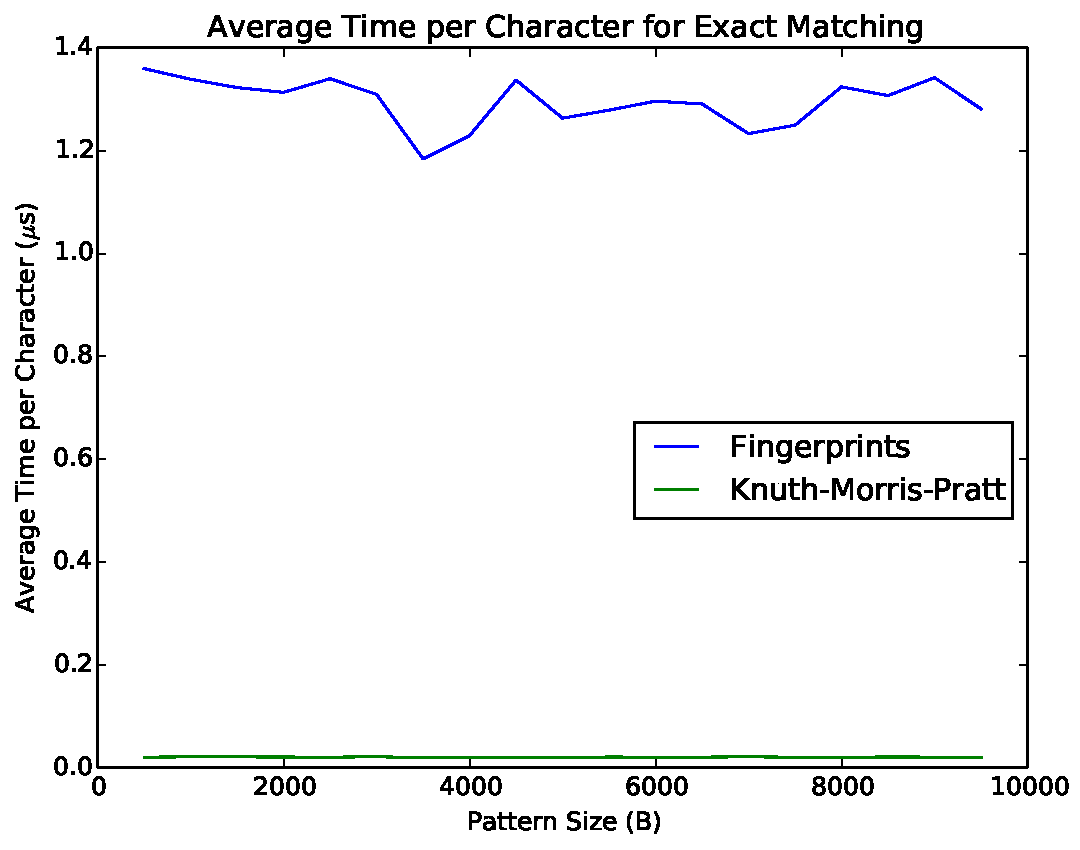
\includegraphics[scale=0.58]{exact_run_time}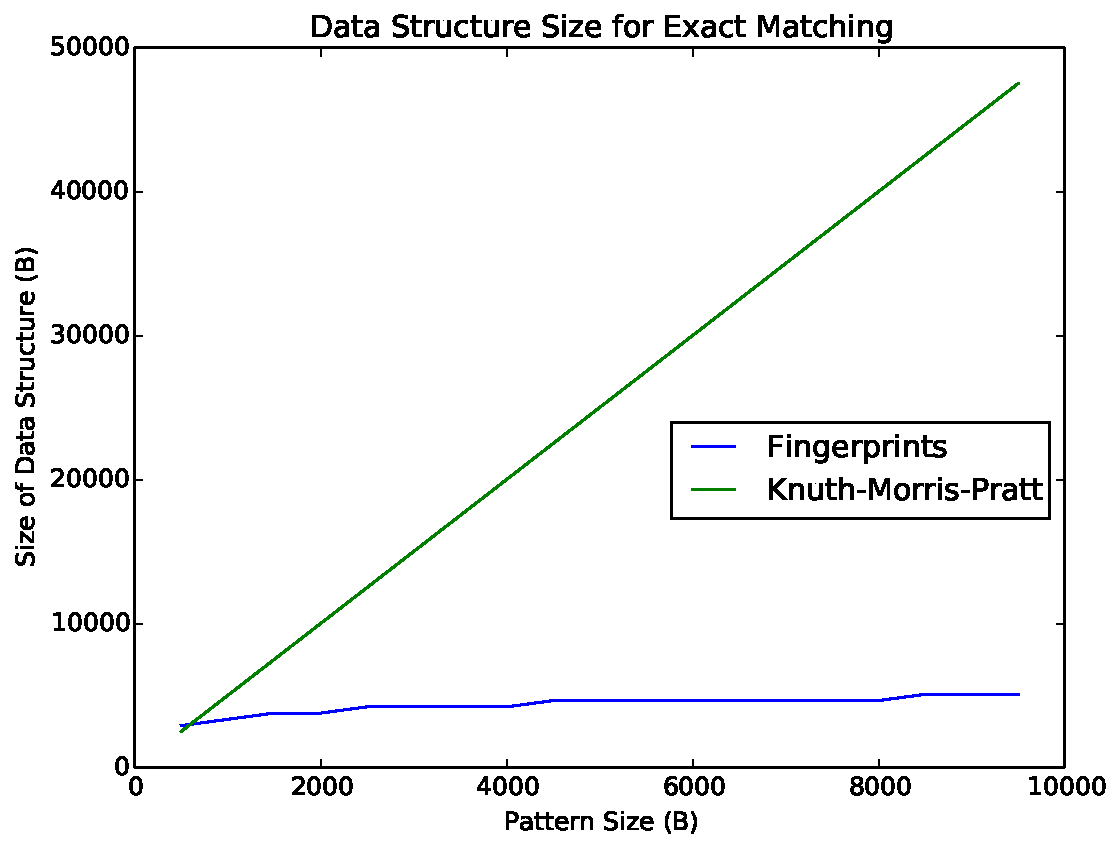
\includegraphics[scale=0.58]{exact_size}
  \end{center}
  \end{block}
  \end{column}
\end{columns}

\vfill

\begin{columns}[t]
  \begin{column}{0.422\linewidth}
  \begin{block}{\Large Parameterised Matching Conclusions}
  The main bottleneck in Parameterised Matching is that previous occurances of characters in the text are stored in a search tree, which takes $O(\log\pi)$ time to query and edit.\\
  \vspace{\baselineskip}
  Question: Can this be improved with dynamic hashing, for which the best results are $O(\sqrt{\log\pi/\log\log\pi})$?
  \end{block}
  \end{column}
  \begin{column}{0.422\linewidth}
  \begin{block}{\Large Exact Matching Conclusions}
  Exact matching with Fingerprints takes 60-70 times longer per character and a significantly longer build time than Knuth-Morris-Pratt, but requires less space than even storing the pattern.\\
  \vspace{\baselineskip}
  Question: The practical bottleneck is that the fingerprints use a lot of modular multiplications. Could these be optimised via precomputation or Montgomery Multiplication?
  \end{block}
  \end{column}
\end{columns}

\vfill

\end{frame}

% -----------------------------------------------------------------------------

\end{document}



